\chapter{EVALUACION Y RESULTADOS}
\section{Especificaciones de la prueba}
Con los conjuntos archivos, se realizo la comparación del algoritmo SCED frente a los algoritmos RKRGST y Winnowing-Fingerprint. El propósito de las pruebas es obtener los resultados sobre el desempeño de los algoritmos, en términos de precisión y tiempo de ejecución en la deteccion de similitud. En la figura \ref{espePrueba} se ilustra el proceso de las pruebas.


\begin{figure}[!h]
\centering
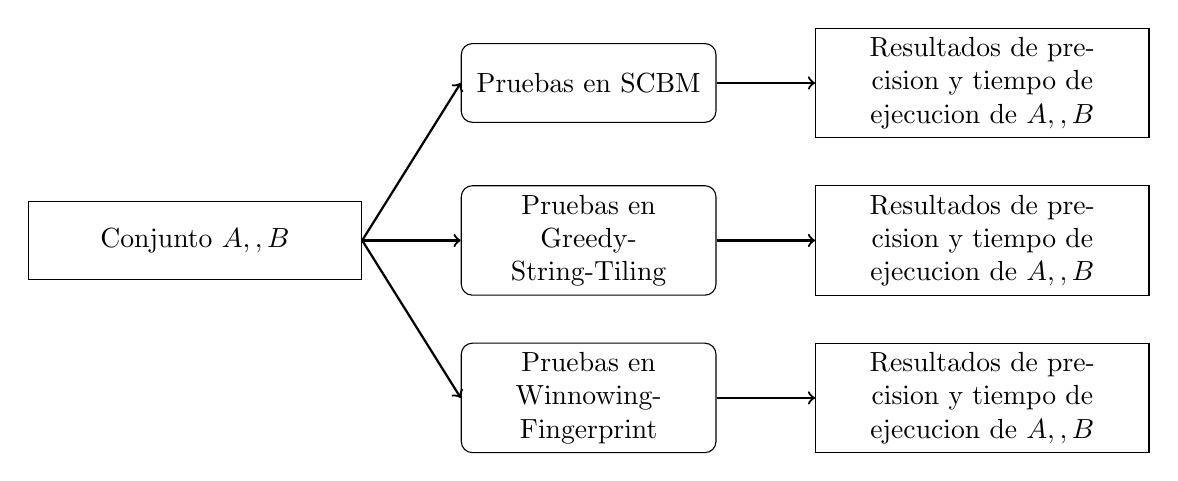
\begin{tikzpicture}[scale=1,
input_output/.style ={rectangle, minimum width=1cm, minimum height=1cm,text centered, text width=4cm, draw=black},
algorithm/.style={rectangle, rounded corners, minimum width=3cm, minimum height=1cm,text centered, text width=3cm, draw=black},
arrow/.style={thick,->,},
]
\node[input_output] (n0) at (1,3) {Conjunto $A, \twodots, B$};
\node[algorithm] (n1) at (6,1) {Pruebas en Winnowing-Fingerprint};
\node[algorithm] (n2) at (6,3) {Pruebas en Greedy-String-Tiling};
\node[algorithm] (n3) at (6,5) {Pruebas en SCBM};
\node[input_output] (n4) at (11,1) {Resultados de precision y tiempo de ejecucion de $A, \twodots, B$};
\node[input_output] (n5) at (11,3) {Resultados de precision y tiempo de ejecucion de $A, \twodots, B$};
\node[input_output] (n6) at (11,5) {Resultados de precision y tiempo de ejecucion de $A, \twodots, B$};
\draw [arrow] (n0.east) to (n1.west);
\draw [arrow] (n0.east) to (n2.west);
\draw [arrow] (n0.east) to (n3.west);
\draw [arrow] (n1.east) to (n4);
\draw [arrow] (n2.east) to (n5);
\draw [arrow] (n3.east) to (n6);
\end{tikzpicture}
\caption{Especificacion de las pruebas}
Fuente: Elaboración propia.
\label{espePrueba}
\end{figure}

\subsection{Pruebas de medicion de precisión en la deteccion de similitud}
En estas prueba se midió la precisión del algoritmo SCED frente a los algoritmos RKRGST y Winnowing-Fingerprint. Para cada para de archivos de un conjunto, se realizó la prueba en complejidad temporal de $O(N^2)$. Es decir para un conjunto, se realizó la comparacion de cada par de archivos del mismo.

La precisión de los algoritmos se determino mediante el porcentaje del indice de similitud entre dos archivos. Los resultados obtenidos de la comparacion de similitud entre archivos del conjunto se almacenó en una matriz, y con escala de grises se observó la similitud que existe. Donde los tonos oscuros representan que existe similitud entre dos archivos y los tonos claros representan lo contrario.

\subsection{Tiempo de ejecucion de las pruebas de medicion}
Con bibliotecas propias del lenguaje de programacion Python se midio el tiempo de ejecucion en segundos de los algoritmos al calcular la similitud en los conjuntos de archivos. La biblioteca utilizada para la medicion fue \id{timeit}. Un ejemplo para la medicion del tiempo de ejecucion de un programa se muestra en el programa \ref{lst:time_it}.

\lstinputlisting[caption={timeit},label={lst:time_it}, language=Python]{programs/time_it.py}

\section{Prueba de medicion Preliminar}
En esta prueba se utilizo los archivos de codigo fuente que se utilizaron en los ejemplos de ofuscacion de codigo fuente, presentados en el marco teorico. En la tabla \ref{firstTest} se muestra el detalle de los programas, el identificador del par y las etiquetas de los programas.

\begin{table}[H]
\centering
\begin{tabular}{|c||c||c|}
\hline
Conjunto & Original & Ofuscado \\ \hline
1 & Programa \ref{lst:obfuscation1_1} & Programa \ref{lst:obfuscation1_2} \\ \hline
2 & Programa \ref{lst:obfuscation2_1} & Programa \ref{lst:obfuscation2_2} \\ \hline
3 & Programa \ref{lst:obfuscation3_1} & Programa \ref{lst:obfuscation3_2} \\ \hline
4 & Programa \ref{lst:obfuscation4_1} & Programa \ref{lst:obfuscation4_2} \\ \hline
5 & Programa \ref{lst:obfuscation5_1} & Programa \ref{lst:obfuscation5_2} \\ \hline
6 & Programa \ref{lst:obfuscation6_1} & Programa \ref{lst:obfuscation6_2} \\ \hline
7 & Programa \ref{lst:obfuscation7_1} & Programa \ref{lst:obfuscation7_2} \\ \hline
8 & Programa \ref{lst:obfuscation8_1} & Programa \ref{lst:obfuscation8_2} \\ \hline
\end{tabular}
\caption{Detalle de los conjuntos de programas con ofuscacion.}
Fuente: Elaboración propia.
\label{firstTest}
\end{table}


En la figura \ref{set_Pre} se muesta los resultados obtenidos en la prueba preliminar.

\begin{figure}[!h]
\centering
\includegraphics[scale=1]{images/results/results_PAIR}
\caption{Resultados de la prueba preliminar}
Fuente: Elaboración propia.
\label{set_Pre}
\end{figure}


\section{Pruebas de medicion en trabajos de catedra}
En estas prueba se utilizo archivos de código fuente en Python enviados por usuarios de un juez de programación. En el cuadro \ref{conjuntoArchivos} se muestra el identificador del conjunto, el numero de problema en el juez, el numero de archivos del conjunto, el promedio de lineas de codigo de los archivos y la varianza de lineas de codigo de los archivos.

\begin{table}[H]
\centering
\begin{tabular}{|c||c|c|c|c|}
\hline
Conjunto & Nro. de Prob. & Nro. de archivos & Prom. de lineas & Var. de lineas \\ \hline \hline
A & 1275  & 10 & 24.8 & 70.84\\ \hline
B & 1407  & 25 & 13.8 & 8.92 \\ \hline
C & 1588  & 41 & 14.24 & 39.84 \\ \hline
D & 1222  & 76 & 2.59 & 0.64 \\ \hline
E & 1089  & 101 & 13.95 & 22.15 \\ \hline
\end{tabular}
\caption{Detalle de los conjuntos de archivos de código fuente para las pruebas}
Fuente: Elaboración propia.
\label{conjuntoArchivos}
\end{table}


\subsection{Prueba de medicion I}
En la prueba I, se midió la precision y el tiempo de ejecucion de los algoritmos con los siguientes parametros:
\begin{itemize}
  \item SCED, $\id{D} = 40$
  \item RKRGST, $\id{threshold} = 80$
  \item Winnowing-Fingerprint, $\id{window-length} = 10, \id{k-grams} = 5$
\end{itemize}

\subsubsection{Conjunto A}
En la figura \ref{set_A_i} se muestra la matriz que se obtuvo para el conjunto A.
\input{figures/set_A_i}

\subsubsection{Conjunto B}
En la figura \ref{set_B_i} se muestra la matriz que se obtuvo para el conjunto B.
\begin{figure}[!h]
\centering
\subfloat[SCED]{
\label{SCED_set_B}
\includegraphics[scale=0.4]{images/results/MAP_1407_SCED_D_40_PRECISION}}
\hspace{-1.5cm}
\subfloat[Greedy-String-Tiling]{
\label{GST_set_B}
\includegraphics[scale=0.4]{images/results/MAP_1407_RKRGST_T_80_PRECISION}}
\hspace{-1.5cm}
\subfloat[Winnowing-Fingerprint]{
\label{WIN_set_B}
\includegraphics[scale=0.4]{images/results/MAP_1407_WIN_W_10_K_5_PRECISION}}
\caption{Prueba de precisión I, conjunto B}
Fuente: Elaboración propia.
\label{set_B_i}
\end{figure}


\subsubsection{Conjunto C}
En la figura \ref{set_C_i} se muestra la matriz que se obtuvo para el conjunto C.
\begin{figure}[!h]
\centering
\subfloat[SCED]{
\label{SCED_set_C}
\includegraphics[scale=0.4]{images/results/MAP_1588_SCED_D_40_PRECISION}}
\hspace{-1.5cm}
\subfloat[RKRGST]{
\label{GST_set_C}
\includegraphics[scale=0.4]{images/results/MAP_1588_RKRGST_T_80_PRECISION}}
\hspace{-1.5cm}
\subfloat[Winnowing-Fingerprint]{
\label{WIN_set_C}
\includegraphics[scale=0.4]{images/results/MAP_1588_WIN_W_10_K_5_PRECISION}}
\caption{Prueba de precisión I, conjunto C}
Fuente: Elaboración propia.
\label{set_C_i}
\end{figure}


\subsubsection{Conjunto D}
En la figura \ref{set_D_i} se muestra la matriz que se obtuvo para el conjunto D.
\begin{figure}[!h]
\centering
\subfloat[SCED]{
\label{SCED_set_D}
\includegraphics[scale=0.4]{images/results/MAP_1222_SCED_D_40_PRECISION}}
\hspace{-1.5cm}
\subfloat[Greedy-String-Tiling]{
\label{GST_set_D}
\includegraphics[scale=0.4]{images/results/MAP_1222_RKRGST_T_80_PRECISION}}
\hspace{-1.5cm}
\subfloat[Winnowing-Fingerprint]{
\label{WIN_set_D}
\includegraphics[scale=0.4]{images/results/MAP_1222_WIN_W_10_K_5_PRECISION}}
\caption{Prueba de precisión I, conjunto D}
Fuente: Elaboración propia.
\label{set_D_i}
\end{figure}


\subsubsection{Conjunto E}
En la figura \ref{set_E_i} se muestra la matriz que se obtuvo para el conjunto E.
\begin{figure}[!h]
\centering
\subfloat[SCED]{
\label{SCED_set_E}
\includegraphics[scale=0.4]{images/results/MAP_1089_SCED_D_40_PRECISION}}
\hspace{-1.5cm}
\subfloat[Greedy-String-Tiling]{
\label{GST_set_E}
\includegraphics[scale=0.4]{images/results/MAP_1089_RKRGST_T_80_PRECISION}}
\hspace{-1.5cm}
\subfloat[Winnowing-Fingerprint]{
\label{WIN_set_E}
\includegraphics[scale=0.4]{images/results/MAP_1089_WIN_W_10_K_5_PRECISION}}
\caption{Prueba de precisión I, conjunto E}
Fuente: Elaboración propia.
\label{set_E_i}
\end{figure}



\subsection{Tiempo de ejecución de la prueba de medicion I}
En la tabla \ref{pruebaTiempoI} se presentan los resultados obtenidos, respecto al tiempo de ejecucion de cada algoritmo al calcular la similitud de cada conjunto de prueba. Los resultados obtenidos se encuentran en segundos.

\begin{table}[H]
\centering
\begin{tabular}{|c|c|ccc|}
\hline
\multirow{2}{*}{Conjunto} & \multirow{2}{*}{Nro. Pares} & \multicolumn{3}{c|}{Prom. tiempo de ejecucion}   \\ \cline{3-5}
                          &                             & \multicolumn{1}{c|}{SCED}  & \multicolumn{1}{c|}{RKRGST}   & WF \\ \hline
A                         & 45                          & \multicolumn{1}{c|}{1.69}  & \multicolumn{1}{c|}{0.90}  & 0.84    \\ \hline
B                         & 300                         & \multicolumn{1}{c|}{4.52}  & \multicolumn{1}{c|}{3.05}  & 3.46    \\ \hline
C                         & 820                         & \multicolumn{1}{c|}{9.93}  & \multicolumn{1}{c|}{7.81}  & 8.65    \\ \hline
D                         & 2850                        & \multicolumn{1}{c|}{19.06} & \multicolumn{1}{c|}{1.90}  & 8.17    \\ \hline
E                         & 5050                        & \multicolumn{1}{c|}{47.76} & \multicolumn{1}{c|}{27.88} & 43.48   \\ \hline
\end{tabular}
\caption{Detalle del promedio de tiempo de ejecución de los algoritmos en la Prueba I.}
Fuente: Elaboración propia.
\label{pruebaTiempoI}
\end{table}


\subsection{Prueba de medicion IV}
En la prueba IV, se midió la precision y el tiempo de ejecucion de los algoritmos con los siguientes parametros:
\begin{itemize}
  \item SCED, $\id{D} = 100$
  \item RKRGST, $\id{threshold} = 20$
  \item Winnowing-Fingerprint, $\id{window-length} = 4, \id{k-grams} = 2$
\end{itemize}

\subsubsection{Conjunto A}
En la figura \ref{set_A_iv} se muestra la matriz que se obtuvo para el conjunto A.
\begin{figure}[!h]
\centering
\subfloat[SCED]{
\label{SCED_set_A}
\includegraphics[scale=0.4]{images/results/MAP_1275_SCED_D_100_PRECISION}}
\hspace{-1.5cm}
\subfloat[Greedy-String-Tiling]{
\label{GST_set_A}
\includegraphics[scale=0.4]{images/results/MAP_1275_RKRGST_T_20_PRECISION}}
\hspace{-1.5cm}
\subfloat[Winnowing-Fingerprint]{
\label{WIN_set_A}
\includegraphics[scale=0.4]{images/results/MAP_1275_WIN_W_4_K_2_PRECISION}}
\caption{Prueba de precisión IV, conjunto A}
Fuente: Elaboración propia.
\label{set_A_iv}
\end{figure}


\subsubsection{Conjunto B}
En la figura \ref{set_B_iv} se muestra la matriz que se obtuvo para el conjunto B.
\begin{figure}[!h]
\centering
\subfloat[SCED]{
\label{SCED_set_B}
\includegraphics[scale=0.4]{images/results/MAP_1407_SCED_D_100_PRECISION}}
\hspace{-1.5cm}
\subfloat[Greedy-String-Tiling]{
\label{GST_set_B}
\includegraphics[scale=0.4]{images/results/MAP_1407_RKRGST_T_20_PRECISION}}
\hspace{-1.5cm}
\subfloat[Winnowing-Fingerprint]{
\label{WIN_set_B}
\includegraphics[scale=0.4]{images/results/MAP_1407_WIN_W_4_K_2_PRECISION}}
\caption{Prueba de precisión IV, conjunto B}
Fuente: Elaboración propia.
\label{set_B_iv}
\end{figure}


\subsubsection{Conjunto C}
En la figura \ref{set_C_iv} se muestra la matriz que se obtuvo para el conjunto C.
\begin{figure}[!h]
\centering
\subfloat[SCED]{
\label{SCED_set_C}
\includegraphics[scale=0.4]{images/results/MAP_1588_SCED_D_100_PRECISION}}
\hspace{-1.5cm}
\subfloat[RKRGST]{
\label{GST_set_C}
\includegraphics[scale=0.4]{images/results/MAP_1588_RKRGST_T_20_PRECISION}}
\hspace{-1.5cm}
\subfloat[Winnowing-Fingerprint]{
\label{WIN_set_C}
\includegraphics[scale=0.4]{images/results/MAP_1588_WIN_W_4_K_2_PRECISION}}
\caption{Prueba de precisión IV, conjunto C}
Fuente: Elaboración propia.
\label{set_C_iv}
\end{figure}


\subsubsection{Conjunto D}
En la figura \ref{set_D_iv} se muestra la matriz que se obtuvo para el conjunto D.
\input{figures/set_D_iv}

\subsubsection{Conjunto E}
En la figura \ref{set_E_iv} se muestra la matriz que se obtuvo para el conjunto E.
\begin{figure}[!h]
\centering
\subfloat[SCED]{
\label{SCED_set_E}
\includegraphics[scale=0.4]{images/results/MAP_1089_SCED_D_100_PRECISION}}
\hspace{-1.5cm}
\subfloat[Greedy-String-Tiling]{
\label{GST_set_E}
\includegraphics[scale=0.4]{images/results/MAP_1089_RKRGST_T_20_PRECISION}}
\hspace{-1.5cm}
\subfloat[Winnowing-Fingerprint]{
\label{WIN_set_E}
\includegraphics[scale=0.4]{images/results/MAP_1089_WIN_W_4_K_2_PRECISION}}
\caption{Prueba de precisión IV, conjunto E}
Fuente: Elaboración propia.
\label{set_E_iv}
\end{figure}



\subsection{Tiempo de ejecución de la prueba de medicion IV}
En la tabla \ref{pruebaTiempoIV} se presentan los resultados obtenidos, respecto al tiempo de ejecucion de cada algoritmo al calcular la similitud de cada conjunto de prueba. Los resultados obtenidos se encuentran en segundos.

\begin{table}[H]
\centering
\begin{tabular}{|c|c|ccc|}
\hline
\multirow{2}{*}{Conjunto} & \multirow{2}{*}{Nro. Pares} & \multicolumn{3}{c|}{Prom. tiempo de ejecucion}   \\ \cline{3-5}
                          &                             & \multicolumn{1}{c|}{SCED}  & \multicolumn{1}{c|}{RKRGST}   & WF \\ \hline
A                         & 45                          & \multicolumn{1}{c|}{1.80}  & \multicolumn{1}{c|}{0.92}  & 0.83    \\ \hline
B                         & 300                         & \multicolumn{1}{c|}{5.11}  & \multicolumn{1}{c|}{3.08}  & 3.59    \\ \hline
C                         & 820                         & \multicolumn{1}{c|}{10.98}  & \multicolumn{1}{c|}{7.92}  & 8.95    \\ \hline
D                         & 2850                        & \multicolumn{1}{c|}{19.20} & \multicolumn{1}{c|}{1.90}  & 9.00    \\ \hline
E                         & 5050                        & \multicolumn{1}{c|}{53.61} & \multicolumn{1}{c|}{28.30} & 47.03   \\ \hline
\end{tabular}
\caption{Detalle del promedio de tiempo de ejecución de los algoritmos en la Prueba IV.}
Fuente: Elaboración propia.
\label{pruebaTiempoIV}
\end{table}


\subsection{Prueba de medicion V}
En la prueba V, se midió la precision y el tiempo de ejecucion del algoritmos de programacion dinamica convencional para el calculo de la distancia de edicion (LEVED) y el algoritmo SCED.

\subsubsection{Conjunto A}
En la figura \ref{set_A_v} se muestra la matriz que se obtuvo para el conjunto A.
\begin{figure}[!h]
\centering
\subfloat[LEVED]{
\label{EDIT_set_A_v}
\includegraphics[scale=0.4]{images/results/MAP_1275_EDIT_D_100_PRECISION}}
%\hspace{-1.5cm}
\subfloat[SCED]{
\label{SCED_set_A_v}
\includegraphics[scale=0.4]{images/results/MAP_1275_SCED_D_100_PRECISION}}
\caption{Resultados de la prueba de similitud del conjunto A}
Fuente: Elaboración propia.
\label{set_A_v}
\end{figure}


\subsubsection{Conjunto B}
En la figura \ref{set_B_v} se muestra la matriz que se obtuvo para el conjunto B.
\begin{figure}[!h]
\centering
\subfloat[LEVED]{
\label{EDIT_set_B_v}
\includegraphics[scale=0.4]{images/results/MAP_1407_EDIT_D_100_PRECISION}}
%\hspace{-1.5cm}
\subfloat[SCED]{
\label{SCED_set_B_v}
\includegraphics[scale=0.4]{images/results/MAP_1407_SCED_D_100_PRECISION}}
\caption{Resultados de la prueba de similitud del conjunto B}
Fuente: Elaboración propia.
\label{set_B_v}
\end{figure}


\subsubsection{Conjunto C}
En la figura \ref{set_C_v} se muestra la matriz que se obtuvo para el conjunto C.
\begin{figure}[!h]
\centering
\subfloat[LEVED]{
\label{EDIT_set_C_v}
\includegraphics[scale=0.4]{images/results/MAP_1588_EDIT_D_100_PRECISION}}
%\hspace{-1.5cm}
\subfloat[SCED]{
\label{SCED_set_C_v}
\includegraphics[scale=0.4]{images/results/MAP_1588_SCED_D_100_PRECISION}}
\caption{Resultados de la prueba de similitud del conjunto C}
Fuente: Elaboración propia.
\label{set_C_v}
\end{figure}


\subsubsection{Conjunto D}
En la figura \ref{set_D_v} se muestra la matriz que se obtuvo para el conjunto D.
\begin{figure}[!h]
\centering
\subfloat[LEVED]{
\label{EDIT_set_D_v}
\includegraphics[scale=0.4]{images/results/MAP_1222_EDIT_D_100_PRECISION}}
%\hspace{-1.5cm}
\subfloat[SCED]{
\label{SCED_set_D_v}
\includegraphics[scale=0.4]{images/results/MAP_1222_SCED_D_100_PRECISION}}
\caption{Resultados de la prueba de similitud del conjunto D}
Fuente: Elaboración propia.
\label{set_D_v}
\end{figure}


\subsubsection{Conjunto E}
En la figura \ref{set_E_v} se muestra la matriz que se obtuvo para el conjunto E.
\begin{figure}[!h]
\centering
\subfloat[LEVED]{
\label{EDIT_set_E_v}
\includegraphics[scale=0.4]{images/results/MAP_1089_EDIT_D_100_PRECISION}}
%\hspace{-1.5cm}
\subfloat[SCED]{
\label{SCED_set_E_v}
\includegraphics[scale=0.4]{images/results/MAP_1089_SCED_D_100_PRECISION}}
\caption{Resultados de la prueba de similitud del conjunto E}
Fuente: Elaboración propia.
\label{set_E_v}
\end{figure}


\subsection{Tiempo de ejecución de la prueba de medicion V}
En la tabla \ref{pruebaTiempoV} se presentan los resultados obtenidos, respecto al tiempo de ejecucion de cada algoritmo al calcular la similitud de cada conjunto de prueba. Los resultados obtenidos se encuentran en segundos.

\begin{table}[H]
\centering
\begin{tabular}{|c|c|cc|}
\hline
\multirow{2}{*}{Conjunto} & \multirow{2}{*}{Nro. Pares} & \multicolumn{2}{c|}{Prom. tiempo de ejecucion}   \\ \cline{3-4}
                          &                             & \multicolumn{1}{c|}{LEVED} & \multicolumn{1}{c|}{SCED} \\ \hline
A                         & 45                          & \multicolumn{1}{c|}{2.81}  & \multicolumn{1}{c|}{1.80}    \\ \hline
B                         & 300                         & \multicolumn{1}{c|}{9.67}  & \multicolumn{1}{c|}{5.11}    \\ \hline
C                         & 820                         & \multicolumn{1}{c|}{27.74}  & \multicolumn{1}{c|}{10.98}  \\ \hline
D                         & 2850                        & \multicolumn{1}{c|}{3.31}  & \multicolumn{1}{c|}{19.20}   \\ \hline
E                         & 5050                        & \multicolumn{1}{c|}{89.27} & \multicolumn{1}{c|}{53.61} \\ \hline
Total                     & 9065                        & \multicolumn{1}{c|}{132.8} & \multicolumn{1}{c|}{90.61}  \\ \hline
\end{tabular}
\caption{Detalle del promedio de tiempo de ejecución de los algoritmos}
Fuente: Elaboración propia.
\label{pruebaTiempoV}
\end{table}


\section{Prueba de hipotesis}
Para la prueba de hipotesis se utilizó como muestra, las mediciones obtenidas en la prueba V por los algoritmos LEVED y SCED en el calculo de similitud sobre los conjuntos A, B, C, D y E. En la tabla \ref{DescTable} se muestra los estadisticos descriptivos de la muestra.

\begin{table}[H]
\centering
\begin{tabular}{c|c|c|c|c|c|}
\cline{2-6}
                                & N    & Media & Desv. estándar & Mínimo & Máximo \\ \hline
\multicolumn{1}{|c|}{LEVED} & 9065 & 52.12 & 21.85          & 13.33   & 100.00 \\ \hline
\multicolumn{1}{|c|}{SCED}      & 9065 & 61.65 & 22.38          & 25.42  & 100.00 \\ \hline
\end{tabular}
\caption{Estadisticos descriptivos de la muestra}
Fuente: Elaboracion propia.
\label{DescTable}
\end{table}


\subsection{Prueba de normalidad}
Antes de escoger el estadistico para la prueba de hipotesis, se debe comprobar si la muestra esta distruida de forma normal, como el numero de datos es grande se utiliza la prueba de normalidad de Kolmogorov-Smirnov. Esta prueba se la realiza con las diferencias entre las mediciones de la muestra, para dos conjuntos de mediciones $A={a_1,a_2,\twodots,a_m}$ y $B={a_1,a_2,\twodots,a_m}$, la diferencia de mediciones esta dado por $C={c_1,c_2,\twodots,c_m}$ donde $c_i = a_i - b_i$.
\begin{itemize}
  \item[] \textbf{Paso 1.} Planteamiento de la hipotesis de normalidad:
  \begin{equation*}
  \begin{split}
  H_0 & = \text{Los datos de la muestra siguen una distribucion normal}\\
  H_1 & = \text{Los datos de la muestra no siguen una distribucion normal}
  \end{split}
  \end{equation*}
  \item[] \textbf{Paso 2.} Nivel de significancia:
  \begin{equation*}
  \begin{split}
  N.C. & = 0.95 \\
  \alpha & = 0.05
  \end{split}
  \end{equation*}
  \item[] \textbf{Paso 3.} Prueba de Nornmalidad:
  \begin{center}
  Si $n > 50$ aplicar la prueba de Kolmogorov-Smirnov.
  \end{center}
  \item[] \textbf{Paso 4.} Criterio de decision:
  \begin{center}
  Si $\text{valor p} < \alpha$ se rechaza $H_0$ y se acepta $H_1$.\\
  Si $\text{valor p} \geq \alpha$ se acepta $H_0$ y se rechaza $H_1$.
  %Si $\id{Z} < Z_\alpha/2$ se rechaza $H_0$ y se acepta $H_1$.\\
  %Si $\id{Z} \geq Z_\alpha/2$ se acepta $H_0$ y se rechaza $H_1$.
  \end{center}
  \item[] \textbf{Paso 5.} Resultados y conclusion.
  Como el tamaño de la muestra es $N=5050$ se aplica la prueba de Kolmogorov-Smirnov y el detalle de los resultados se muestra en la tabla \ref{KStable}.
  \begin{table}[H]
\centering
\begin{tabular}{c|c|c|c|}
\cline{2-4}
                                & Estadistico & g.l. & Valor p \\ \hline
\multicolumn{1}{|c|}{C} & 0.048        & 9065 & 0.001    \\ \hline
\end{tabular}
\caption{Estadistico de Kolmogorov-Smirnov}
Fuente: Elaboracion propia.
\label{KStable}
\end{table}

  Para el valor p obtenido se tiene que $0.001 < 0.05$, entonces se rechaza $H_0$ y se acepta $H_1$. Con el rechazo de hipotesis nula y se aceptacion de la hipotesis de alterna, se puede inferir que los datos no siguen una distribucion normal.
\end{itemize}

Con esta prueba de normalidad aseguramos que el estadistico para contrastar la hipotesis debe tener enfoque no parametrico.

\subsection{Prueba de los rangos con signo de Wilcoxon}
La prueba de Wilcoxon es una prueba no parametrica alternativa a la prueba T para dos muestras relacionadas, es decir los resultados del primer conjunto no son independientes del segundo conjunto, dado que ambas mediciones se obtuvieron de una misma muestra. Se la utiliza para determinar si la diferencia de medianas de mediciones relacionadas se debe al azar o no. El estadistico se muestra en la siguiente ecuacion \ref{disWil}. Los supuestos para esta prueba son: Los datos deben ser dependientes, los datos deben estar medidos a nivel ordinal, no requiere que los datos se distribuyan de forma normal.

\begin{equation}
Z = \frac{W-n(n+1)/4}{\sqrt{n(n+1)(2n+1)/24}}
\label{disWil}
\end{equation}

\subsubsection{Calculo de W}
El procedimento para obtener el valor \id{W} es el siguiente:
\begin{itemize}
  \item Calcular las diferencias entre las dos puntuaciones de cada pareja.
  \begin{equation*}
    z_i = x_i - y_i
  \end{equation*}
  \item Calcular el valor absoluto de las diferencias de cada pareja.
  \begin{equation*}
    z_i = |x_i - y_i|
  \end{equation*}
  \item Ordenar los valores absolutos $|z_1|,|z_2|,\twodots,|z_n|$ y asignar su rango. El rango $R_i$ de un número es el tamaño relativo a otros valores en la lista.
  \item Calcular los estadisticos de prueba de Wilcoxon $W^{+}$ y $W^{+}$.
  \begin{equation*}
  \begin{split}
  W^{+} & = \sum_{z_i>0}{R_i} \\
  W^{-} & = \sum_{z_i<0}{R_i}
  \end{split}
  \end{equation*}
  \item Calcular el minimo valor entre $W^{+}$ y $W^{-}$.
  \begin{equation*}
    W=\proc{min}(W^{+}, W^{-})
  \end{equation*}
\end{itemize}

\subsubsection{Prueba de Wilcoxon}
La hipotesis planteada en la investigacion indica que: ``El algoritmo SCED detecta la similitud entre códigos fuente con una confiabilidad del 95\% frente al algoritmo convencional que calcula la distancia de Levenshtein''. Donde las variables que fueron evaluadas son las siguientes:
\begin{itemize}
  \item[] \textbf{Variable independiente:} El diseño del algoritmo \id{SCED}
  \item[] \textbf{Variable dependiente:} Resultados en la deteccion de similitud entre codigos fuente con una confiabilidad del 95\% frente a los algoritmo de RKRGST y Winnowing-Fingerprint.
\end{itemize}

El procedimento para contrastar la hipotesis de investigacion es el siguiente:
\begin{itemize}
  \item[] \textbf{Paso 1.} Planteamiento de la hipotesis:
  \begin{equation*}
  \begin{split}
  H_0 & = \mu_d = 0 \\
  H_1 & = \mu_d < 0
  \end{split}
  \end{equation*}
  \item[] \textbf{Paso 2.} Nivel de significancia:
  \begin{equation*}
  \begin{split}
  N.C. & = 0.95 \\
  \alpha & = 0.05
  \end{split}
  \end{equation*}
  \item[] \textbf{Paso 3.} Criterio de decision:
  \begin{center}
  Si $\id{Z} < Z_\alpha$ se rechaza $H_0$ y se acepta $H_1$\\
  Si $\id{Z} \geq Z_\alpha$ se acepta $H_0$ y se rechaza $H_1$
  %Si $\id{valor-p} < \alpha$ se rechaza $H_0$ y se acepta $H_1$\\
  %Si $\id{valor-p} \geq \alpha$ se acepta $H_0$ y se rechaza $H_1$
  \end{center}
  \item[] \textbf{Paso 4.} Resultados y conclusion.\\
  Se aplica la prueba de Wilcoxon a la muestra, el detalle de los resultados se muestra en la tabla \ref{wilTable}.
  \begin{table}[H]
\centering
\begin{tabular}{c|c|c|c|}
\cline{2-4}
                                       & N    & Rango prom. & Suma de rangos \\ \hline
\multicolumn{1}{|c|}{Rangos negativos $(W_{-})$} & 1114 & 3080.62     & 3431815.00     \\ \hline
\multicolumn{1}{|c|}{Rangos positivos $(W_{+})$} & 7826 & 4668.34     & 36534455.00    \\ \hline
\multicolumn{1}{|c|}{Empates}          & 125 & -           & -              \\ \hline
\multicolumn{1}{|c|}{Total}            & 9065 & -           & -              \\ \hline
\end{tabular}
\caption{Rangos de la prueba de Wilcoxon}
Los rangos negativos, positivos y empates representan: $\id{SCED}<\id{LEVED}$, $\id{SCED}>\id{LEVED}$ y $\id{SCED}=\id{LEVED}$.
Fuente: Elaboracion propia.
\label{rangTable}
\end{table}

  \begin{table}[H]
\centering
\begin{tabular}{c|c|}
\cline{2-2}
                              & LEVED - SCED \\ \hline
\multicolumn{1}{|c|}{Z}       & -67.82          \\ \hline
\multicolumn{1}{|c|}{valor-p} & 0.00           \\ \hline
\end{tabular}
\caption{Prueba de rangos con signo de Wilcoxon}
El estadistico \id{Z} se basa en rangos negativos.
Fuente: Elaboracion propia.
\label{wilTable}
\end{table}

  Para los valores obtenidos se tiene que $-67.82 < -1.64$, entonces se rechaza $H_0$ y se acepta $H_1$. Ademas el $\text{valor p} < \alpha$ indica que los datos son poco probables con una hipotesis nula verdadera. Con el rechazo de hipotesis nula y se aceptacion de la hipotesis de alterna, se puede inferir que el algoritmo SCED detecta similitud entre codigos fuente con una confiabilidad del 95\% frente al algoritmo convencional que calcula la distancia de edicion.
\end{itemize}
